

\section{Preshower detectors}


%%%%%% SLIDE
\begin{frame}{\textcolor{Goldenrod}{Preshower detector }}
  \begin{overlayarea}{\textwidth}{\textheight}
    \(
    \<{0.35\textwidth}
    %\begin{figure}[h]\centering
      \img{33_PS}\\
      \img{31_PS}\\
      % 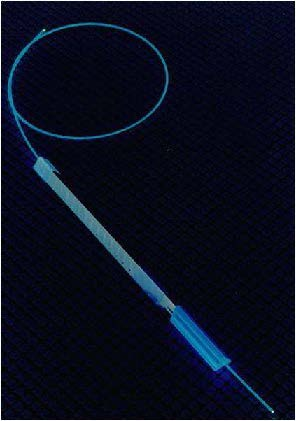
\includegraphics[height=0.4\textheight]{./Images/32_PS}
    %\end{figure}
    \>
    \<{0.75\textwidth}
    \itt[<+->]
  \item triangular strips of
    scintillator
  \item calorimeters as well as tracking detectors
  \item electron ID and background
    rejection at online triggering and offline reconstruction.
  \item The central preshower detector
    (CPS) consisted of three concentric cylindrical layers ($|\eta| <
    1.3$)
    % and is located between the solenoid and the central calorimeter
  \item The two forward preshower detectors (FPS) cover $1.5 < |\eta| < 2.5$
    % and are attached to the faces of the end calorimeters.
  \item a wavelength-shifter at center of each strip
    \tti
    
    \note{, enhancing the
      spatial matching be- tween tracks and calorimeter showers [78]. The
      detectors can be used offline to correct the electromagnetic energy
      measurement of the central and end calorimeters for losses in the
      solenoid and upstream material}
    
    \note{Since the triangles are
      interleaved, there is no dead space between strips and most tracks
      traverse more than one strip, allowing for strip-to-strip
      interpolations and improved position measurement.}

    \note{The preshower detectors share common elements with the central
      fiber tracker, beginning with the waveguides and continuing
      through the entire readout elec- tronics system.}
    \>   
    \)
  \end{overlayarea}
\end{frame}


%%%%%% SLIDE
\begin{frame}{\textcolor{Goldenrod}{Forward Preshower detector }}
  \(
  \<{0.75\textwidth}
  \itt[<+->]
\item[$\bullet$] The upstream layers are known as the minimum ionizing particle,
  or MIP, layers while the downstream layers behind the absorber are
  called the shower layers.
\item[$\bullet$] Charged particles passing through the detector will register
  minimum ionizing signals in the MIP layer $\to$ tracking.
  
\item[$\bullet$] {\small Electrons shower in the absorber $\to$ a cluster of
  energy,
  % (typically on the order of three strips wide),
  which is then matched
  to MIP-layer signal.}
  
\item[$\bullet$] {\small Photons will not generally interact in the MIP layer, but will
  produce a shower signal in the shower layer.}
  
\item[$\bullet$] {\small Heavier charged particles are less likely to shower, typically
  producing a second MIP signal in the shower layer.}
  \tti
  \>
  \<{0.4\textwidth}
  \img{30_PS}\\
  {\scriptsize FPS module with  $u -v$ MIP
    and shower layers, separated by a lead and stainless steel absorber.}
  \>
  \)
\end{frame}

%%%%%%SLIDE
\begin{frame}{\textcolor{Goldenrod}{Title}}
  \(
  \<{0.6\textwidth}
  \itt[<+->]
\item item 
  \item
    \tti
  \>
  
  \<{0.4\textwidth}
  % \img{}
  \>
  \)
\end{frame}

%%%%%%%%% SLIDE
% \begin{frame}{\textcolor{Goldenrod}{Title }}
%   \begin{figure} \centering
%     %%%% figure manipulation 
%     \begin{tikzpicture}[zoomboxarray,connect zoomboxes, zoombox paths/.append style={ultra thick, red}]
%       \node [image node, help grid]
%       { 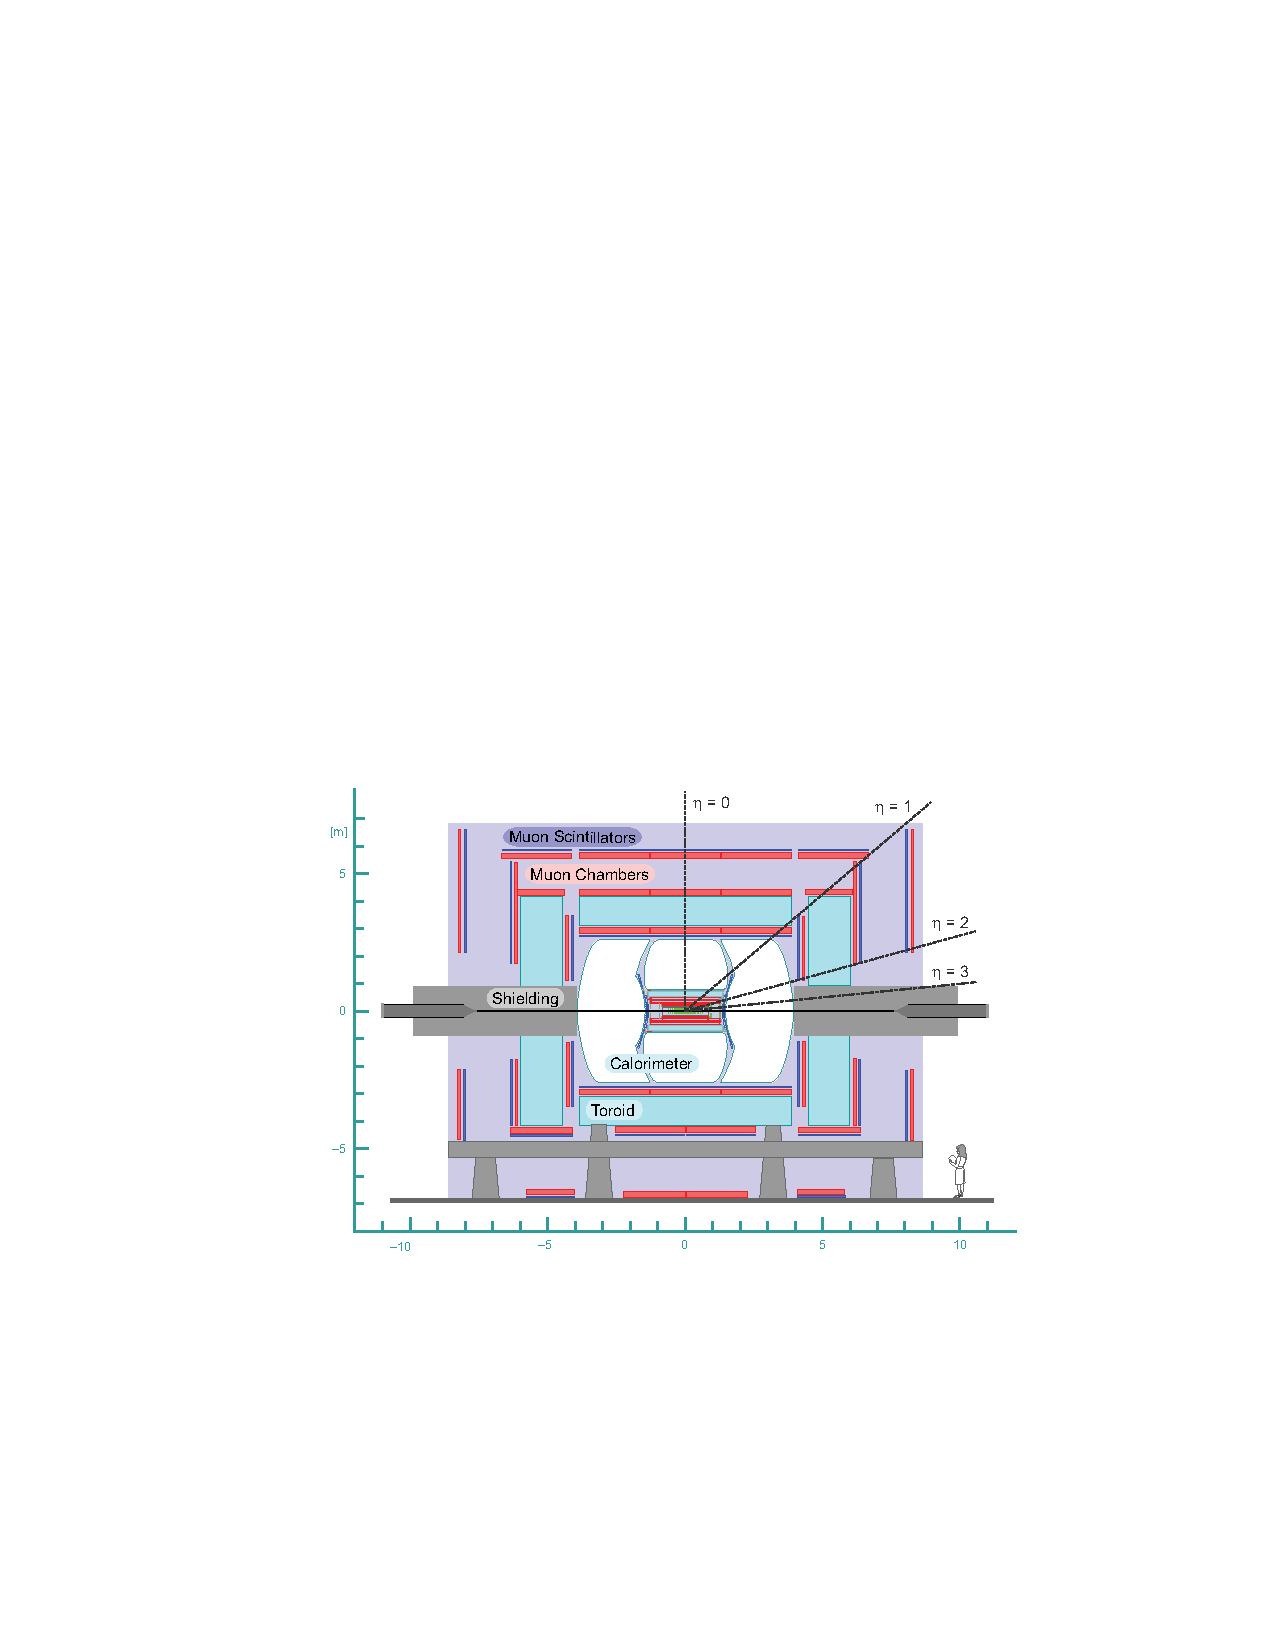
\includegraphics[width=0.45\textwidth]{./Images/01_dzero_wholedetector.pdf}};
%       \onslide<2->\zoombox[magnification=5,color code=lime]{0.86,0.35}
%     \end{tikzpicture}
%   \end{figure}
% \end{frame}  
\end{document}


\subsection{Central preshower detector}
\subsection{Forward preshower detector}
